\chapter{Discussion}
\label{sec:discussion}
Etwas Text... Hier kommen noch einige Abkürzunge vor zum Beispiel \ac{ABC},\ac{WWW} und \ac{ROFL}.

\section{Erste Überschrift Tiefe 2 (section)}
blindtext

\subsection{Erste Überschrift Tiefe 3 (subsection)}
blindtext

\subsubsection{Erste Überschrift Tiefe 4 (subsubsection)}
blindtext

\begin{figure}[H]
    \centering
    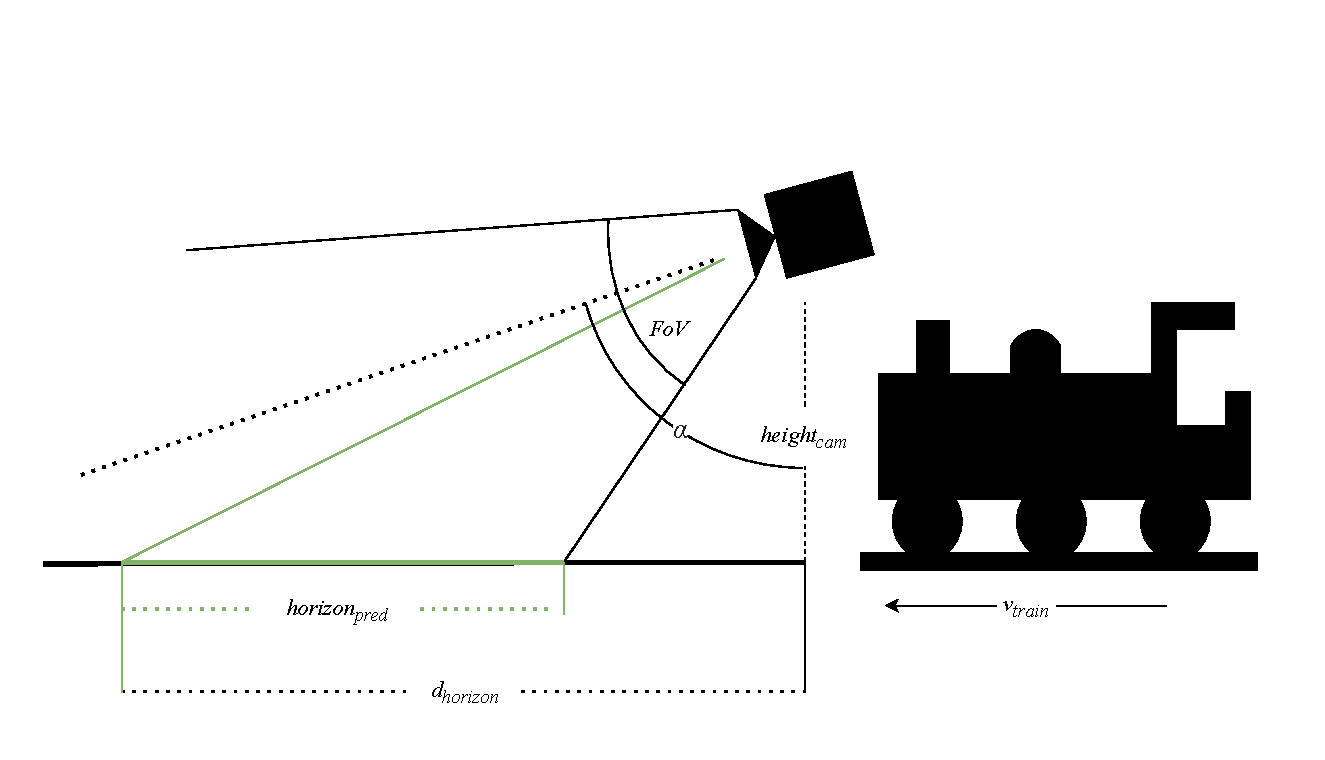
\includegraphics[width=0.8\textwidth]{PICs/discussion/Kameraaufbau.pdf}
    \caption{Camerasetup}
    \label{fig:cameraSetup}
\end{figure}

\begin{align}
    FPS = \frac{v_{train}}{d_{horizon}} \times \frac{1}{\lambda}
    \label{func:RealTime}
\end{align}

<bild von einer prediction um zu zeigen dass es ca 1/3 des bildes ausmacht -> \autoref{fig:autocropVideoComparison} 

\begin{table}[H]
    \centering
    \begin{tabular}{|l|c|c|}
    %\begin{tabular}{| p{0.3\linewidth} | p{0.6\linewidth} |}
        \hline
        \textbf{Parameters} & \textbf{Variables} & \textbf{Assumptions}\\
        \hline
        Camera model & & GoPro Hero 10 Black \cite{goproHero10} \\
        \hline
        Vertical Field of View & $FoV$ & $93^\circ$ \cite{goproHero10} \\
        \hline
        Camera mounting angle & $\alpha$ & $90^\circ$ \\
        \hline
        Camera mounting height & $height_{cam}$ & 4 m \\
        \hline
        Train speed & $v_{train}$ & 265 km/h \cite{geschwindigkeitZugAustria} $ \Leftrightarrow\ $ 73.61 m/s\\
        \hline
        Predicted horizon line & $ horizon_{pred} $ & 480 pixel from top \\
        \hline
        Overlap factor & $\lambda$ & 0.17 \\
        \hline
    \end{tabular}
    \caption{Variables for real time calculation}
    \label{tab:variablesForRealTime}
\end{table}

\begin{align}
    l_{blind} = \tan \left( \alpha-\frac{FoV}{2} \right) \times height_{cam} = \tan \left( 90^\circ-\frac{93^\circ}{2} \right) \times 3 = 2.85 \, {m}
    \label{func:lBlind}
\end{align}

\begin{align}
    d_{horizon} = \tan \left( \left( \frac{image_{height} - horizon_{pred}}{image_{height}} \times FoV \right) + \alpha - \frac{FoV}{2} \right) \times height_{cam}
    \label{func:dHorizon}
\end{align}

\begin{align}
    d_{horizon} = \tan \left( \left( \frac{720 - 480}{720} \times 93 \right) + 90 - \frac{93}{2} \right) \times 4 = 14.42 \, {m}
    \label{func:dHorizonValues}
\end{align}

\begin{align}
    FPS = \frac{v_{train}}{d_{horizon}} \times \frac{1}{\lambda} = \frac{73.61}{14.42} \times \frac{1}{1} = 5.1
    \label{func:FPSValues}
\end{align}

\begin{align}
    FPS = \frac{v_{train}}{d_{horizon}} \times \frac{1}{\lambda} = \frac{73.61}{14.42} \times \frac{1}{0.17} = 30
    \label{func:FPSValuesOverlap}
\end{align}

\begin{align}
    d_{frames} = \frac{v_{train}}{FPS} = \frac{73.61}{30} = 2.45 \, {m}
    \label{func:distanceBetweenFrameswith30FPS}
\end{align}

\vspace{1cm}

\begin{figure}[H]
    \centering
    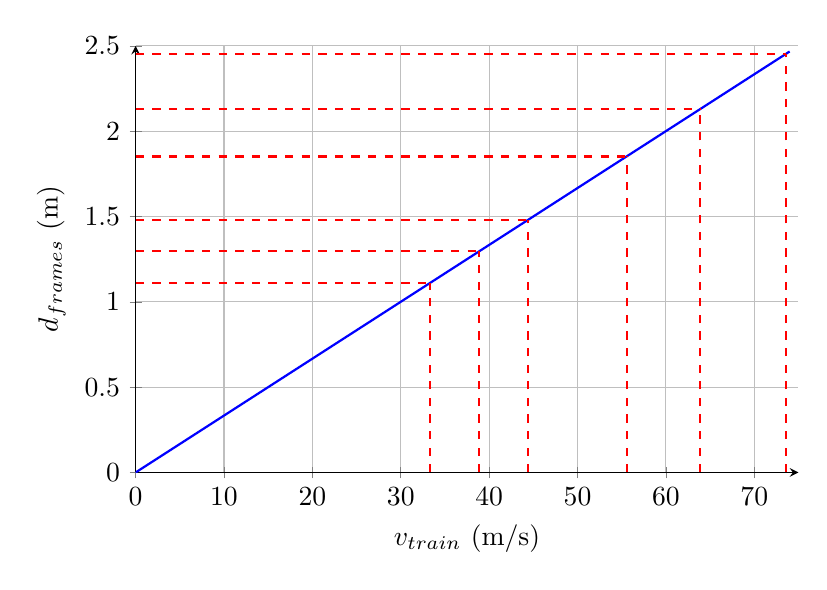
\begin{tikzpicture}
    \begin{axis}[
        width=10cm, height=7cm, % Größe des Graphen
        xlabel={$v_{train}$ (m/s)},
        ylabel={$d_{frames}$ (m)},
        xmin=0, xmax=75, % Begrenzung der x-Achse
        ymin=0, ymax=2.5, % Begrenzung der y-Achse
        grid=major,
        axis lines=left,
        legend style={at={(0.95,0.05)},anchor=south east},
        ]
        % Graph der Funktion y = 1/30 * x
        \addplot[blue, thick, domain=0:74, samples=100] {1/30 * x};
        
        % Vertikale und horizontale Linien für die gewünschten Geschwindigkeiten
        % 120 km/h = 33.33 m/s
        \draw[red, thick, dashed] (axis cs:33.33,0) -- (axis cs:33.33,1.111); % vertikal
        \draw[red, thick, dashed] (axis cs:0,1.111) -- (axis cs:33.33,1.111); % horizontal
        
        % 140 km/h = 38.89 m/s
        \draw[red, thick, dashed] (axis cs:38.89,0) -- (axis cs:38.89,1.2963); % vertikal
        \draw[red, thick, dashed] (axis cs:0,1.2963) -- (axis cs:38.89,1.2963); % horizontal
        
        % 160 km/h = 44.44 m/s
        \draw[red, thick, dashed] (axis cs:44.44,0) -- (axis cs:44.44,1.4813); % vertikal
        \draw[red, thick, dashed] (axis cs:0,1.4813) -- (axis cs:44.44,1.4813); % horizontal
        
        % 200 km/h = 55.56 m/s
        \draw[red, thick, dashed] (axis cs:55.56,0) -- (axis cs:55.56,1.8519); % vertikal
        \draw[red, thick, dashed] (axis cs:0,1.8519) -- (axis cs:55.56,1.8519); % horizontal
        
        % 230 km/h = 63.89 m/s
        \draw[red, thick, dashed] (axis cs:63.89,0) -- (axis cs:63.89,2.1297); % vertikal
        \draw[red, thick, dashed] (axis cs:0,2.1297) -- (axis cs:63.89,2.1297); % horizontal
        
        % 265 km/h = 73.61 m/s
        \draw[red, thick, dashed] (axis cs:73.61,0) -- (axis cs:73.61,2.4537); % vertikal
        \draw[red, thick, dashed] (axis cs:0,2.4537) -- (axis cs:73.61,2.4537); % horizontal
        
    \end{axis}
    \end{tikzpicture}
    \caption{Ratio between the train's speed and the distance it drives between frames with 30 \ac{FPS}. Red lines are top speeds of all different trains from Austria: 120 km/h, 140 km/h, 160 km/h, 200 km/h, 230 km/h, 265 km/h, \cite{geschwindigkeitAllTrainsAustria}}
    \label{fig:ratioSpeedDistanceBetweenFrames}
\end{figure}
